\documentclass[notheorems, aspectratio=169, 12pt, unicode]{beamer}
\usepackage{mysettings}
\begin{document}

\begin{frame}
 \titlepage
\end{frame}

 \section{Introduction}
 
 \begin{frame}<handout:0>{自己紹介}
  \begin{itemize}
   \item PN : そくらてす
   \item 普段やっていること : \pause
	 \begin{itemize}
	  \item 某大学計算機科学系の学科の博士課程の学生
		\begin{itemize}
		 \item \alert{計算機科学何もわからん(ノдヽ)} \pause
		 \item \alert{数学何もわからん(ノдヽ)} \pause
		 \item \alert{任意の概念何もわからん(ノдヽ)} \pause
		 \item けんきゅーしてること : 証明論のようなもの \pause
		\end{itemize}
	  \item \structure{Twitter} でくだを巻く \pause 
	 \end{itemize}
   \item 間違ったこと言ったら教えてね
  \end{itemize} 
 \end{frame}
 
 \section{Separation Logic}

 \begin{frame}{分離論理とは?}
  \begin{itemize}
   \item \alert{分離論理}とは? \pause
	 \begin{itemize}
	  \item \alert{ヒープ領域}に言及できる論理体系
	  \item \alert{ヒープ領域}の状態を表す記法 \pause
	 \end{itemize}
   \item \alert{ヒープ領域}とは? \pause
	 \begin{itemize}
	  \item C言語などの\alert{ポインタ}で触ることのできるメモリの領域 \pause
		(と思っといてくれ) 
	 \end{itemize}
  \end{itemize} 
 \end{frame}

 \begin{frame}{分離論理の論理式}
 \begin{definition}[分離論理の論理式]
  \minusbaselineskip
  \begin{align*}
   &\text{Variables(変数記号)}  &x &\in \mathVar \\
   &\text{Terms(項)}  &t &::= \mathvalnil \mathrelbar x \\
   &\text{Atomic Formul\ae(原子論理式)}  &\alpha &::= \mathemp \mathrelbar  t = t  \mathrelbar \alert{\mathpointer{t}{1}{t}} \mathrelbar  \alert{\mathpointer{t}{2}{t{,}\ t}} \mathrelbar \\
   & & &\phantom{{}::={}}  \alert{\mathprls{t}{t}} \mathrelbar \alert{\mathprtree{t}}  \\
   &\text{Formul\ae(論理式)}  &\varphi &::= \alpha \mathrelbar \lnot \varphi \mathrelbar \varphi \land \varphi \mathrelbar \exists x.\varphi \mathrelbar \alert{\varphi \mathsepstar \varphi} \mathrelbar \alert{\varphi \mathmagicwand \varphi} \\
  \end{align*}
 \end{definition}
 \end{frame}

 \begin{frame}{分離論理の意味のイメージ}{$\mapsto$}
  \begin{table}[tbh]
   \begin{tabular}{cc}
    \begin{minipage}{0.3\hsize}
     \begin{center}
      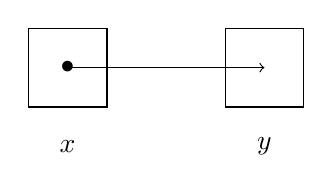
\begin{tikzpicture}
       \draw (0,0) rectangle +(1,1);
       \draw (2.5,0) rectangle +(1,1);
       \draw (0.5,0.5) node{$\bullet$};
       \draw[->] (0.5,0.5) -- (3.0,0.5); 
       \draw (0.5,-0.5) node{$\mathprogramsy{x}$};
       \draw (3.0,-0.5) node{$\mathprogramsy{y}$};
       % \draw (1.5,-1.0) node{$\mathpointer{x}{1}{y}$};
      \end{tikzpicture}
     \end{center}     
    \end{minipage}       
     &
     \begin{minipage}{0.3\hsize}
      \begin{center}
       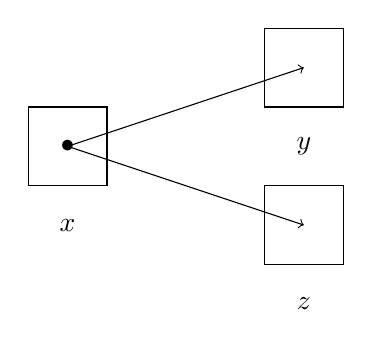
\begin{tikzpicture}
        \draw (-0.5,-0.5) rectangle +(1,1);
        \draw (2.5,0.5) rectangle +(1,1);
        \draw (2.5,-1.5) rectangle +(1,1);

	\draw (0.0,0.0) node{$\bullet$};
	\draw[->] (0.0,0.0) -- (3.0,1.0);
	\draw[->] (0.0,0.0) -- (3.0,-1.0);

        \draw (0.0,-1.0) node{$\mathprogramsy{x}$};
        \draw (3.0,-0.0) node{$\mathprogramsy{y}$};
        \draw (3.0,-2.0) node{$\mathprogramsy{z}$};
       % \draw (1.5,-2.5) node{$\mathpointer{\mathprogramsy{x}}{2}{\mathprogramsy{y}{,}\ \mathprogramsy{z}}$};
       \end{tikzpicture}
      \end{center}
     \end{minipage} \\
     $\mathpointer{x}{1}{y}$ & $\mathpointer{\mathprogramsy{x}}{2}{\mathprogramsy{y}{,}\ \mathprogramsy{z}}$
   \end{tabular}
  \end{table} 
 \end{frame}

\begin{frame}{分離論理の意味のイメージ}{$\mathsepstar$}
  \begin{table}[tbh]
    \begin{tabular}{c}
      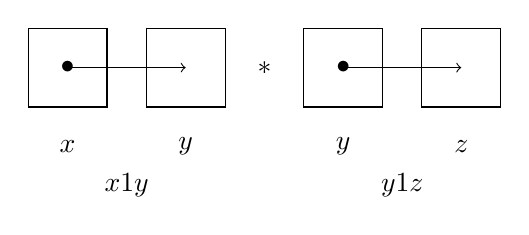
\begin{tikzpicture}
        \draw (0,0) rectangle +(1,1);
        \draw (1.5,0) rectangle +(1,1);
        \draw (0.5,0.5) node{$\bullet$};
        \draw[->] (0.5,0.5) -- (2.0,0.5); 
        \draw (0.5,-0.5) node{$x$};
        \draw (2.0,-0.5) node{$y$};
        \draw (1.25,-1.0) node{$\mathpointer{x}{1}{y}$};
        
        \onslide<2->{\draw (3.0,0.5) node{$*$};}
        
        \draw (3.5,0) rectangle +(1,1);
        \draw (5.0,0) rectangle +(1,1);
        \draw (4.0,0.5) node{$\bullet$};
        \draw[->] (4.0,0.5) -- (5.5,0.5); 
        \draw (4.0,-0.5) node{$y$};
        \draw (5.5,-0.5) node{$z$};
        \draw (4.75,-1.0) node{$\mathpointer{y}{1}{z}$};
      \end{tikzpicture}
       \\
      \onslide<3->
      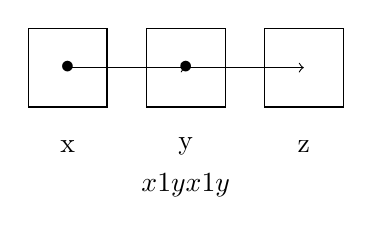
\begin{tikzpicture}
        \draw (0,0) rectangle +(1,1);
        \draw (1.5,0) rectangle +(1,1);
        \draw (3.0,0) rectangle +(1,1);

        \draw (0.5,-0.5) node{x};
        \draw (2.0,-0.5) node{y};
        \draw (3.5,-0.5) node{z};

        \draw (0.5,0.5) node{$\bullet$};
        \draw[->] (0.5,0.5) -- (2.0,0.5);
        \draw (2.0,0.5) node{$\bullet$};
        \draw[->] (2.0,0.5) -- (3.5,0.5);

        \draw (2.0,-1.0) node{$\mathpointer{x}{1}{y}\mathsepstar \mathpointer{x}{1}{y}$};
      \end{tikzpicture}
    \end{tabular}
  \end{table}
\end{frame}

\begin{frame}{分離論理の意味のイメージ}{$\mathprls{\mathdash}{\mathdash}$}
 
\end{frame}

\begin{frame}{分離論理の意味のイメージ}{$\mathprtree{\mathdash}$}
 
\end{frame}

\begin{frame}{分離論理の意味のイメージ}{$\mathmagicwand$}
 
\end{frame}

\section{Program verification}

\begin{frame}{プログラム検証とは?}
 
\end{frame}

\begin{frame}{プログラム検証の例}
 
\end{frame}

\section{References}

\begin{frame}{参考文献}
 \begin{thebibliography}{9}
  \bibitem{Reynolds2002} John C. Reynolds, ``Separation Logic: A Logic for Shared Mutable Data Structure'', Proceedings of the 17th Anual IEEE Symposium on Logic in Computer Science, 2002.
  \bibitem{Brotherston2015} James Brotherston, 
	  `` An introduction to separation logic '', 
	  Logic Summer School, ANU, 7 December 2015.
\bibitem{Sokratesnil2020} Sokratesnil,『分離論理入門のようなもの』,\url{}
 \end{thebibliography} 
\end{frame}

\appendix

\begin{frame}{Frame Rule}
 
\end{frame}

\begin{frame}{Symbolic heap}
  \begin{definition}[Symbolic heap]
  \minusbaselineskip
  \begin{align*}
   &\text{Variables}  &x &\in \mathVar \\
   &\text{Terms}  &t &::= \mathvalnil \mathrelbar x \\
   &\text{Pure Formul\ae}  &\Pi &::=   t = t  \mathrelbar t \neq t \mathrelbar \top \mathrelbar \bot \mathrelbar \Pi \land \Pi \\
   &\text{Spatial Formul\ae}  &\Sigma &::= \mathemp \mathrelbar \mathpointer{t}{1}{t} \mathrelbar  \mathpointer{t}{2}{t{,}\ t} \mathrelbar  \mathprls{t}{t} \mathrelbar \mathprtree{t} \mathrelbar \Sigma \mathsepstar \Sigma \\
   &\text{Formul\ae}  &\varphi &::=  \Pi \land \Sigma
  \end{align*}
 \end{definition}
\end{frame}

\end{document}
